%****************************************************************************
%** Copyright 2002 by Lukas Ruf, ruf@topsy.net
%** Information is provided under the terms of the
%** GNU Free Documentation License http://www.gnu.org/copyleft/fdl.html
%** Fairness: Cite the source of information, visit http://www.topsy.net
%****************************************************************************
%****************************************************************************
%** Last Modification: 2005-07-11 1600
%** 2005-07-11	Bernhard Tellenbach
%**							This is an addapted version of the Introduction.tex file
%**							Added table example (footnotes,multicolumn)
%**							Examples for different text sizes
%**							Updated eps file inclusion example for use with graphicx pkt. 
%****************************************************************************

\chapter{\label{chapter2}Background}

In this chapter, we give a brief overview of BGP in \ref{chapter2:BGP} and explain the problem of long convergence time upon remote failure in BGP. We highlight the architecture and key insights of both iSDX and Swift in \ref{chapter2:iSDX} and \ref{chapter2:Swift}, respectively. The architecture of both frameworks are very similar, they are based on a SDN switch, an SDN controller and a route server. In the next chapter, we explain how these similarities can be put to use in the implementation.

\section{\label{chapter2:BGP}BGP}

The Border Gateway Protocol allows autonomous systems to exchange routing information with each other. The routing information is communicated on a per prefix basis using BGP updates. BGP updates contain the prefix and the AS-path the packet will traverse, if packets are sent via this route. There are two types of updates, announcements and withdraws. Announcements inform that the prefix can be reached via this route and withdraws inform that the prefix can not be reached anymore via this route. \\
Upon receiving a BGP update routers compute the best route to the prefix of the update and then send updates to their peers. Routers only send announcements with their own best route to the prefix and if the routers do not know a route to the prefix they send withdraws.  \\
Convergence time in BGP upon remote failure is slow.
This is because of the way updates propagate trough the network. Changes are only passed on once routers have finished computing the best route to the prefix. Only once all the changes have been received, can routers make sure packets do no get sent into a black hole or loop anymore.



\section{\label{chapter2:iSDX}iSDX}

The iSDX is an internet exchange point enhanced with a SDN switch and SDN controller.\\
An internet exchange point is a physical location where multiple autonomous systems meet to exchange traffic and BGP routes. In a traditional exchange point participants can only use a single route per prefix even though they often have multiple routes available. The iSDX gives the participants additional more fine-grained control over routing decisions. Participants can define policies to make use of this.  \\
In this section we will first show the iSDX architecture in \ref{chapter2:iSDX:iSDX_architecture}, explain the policies in \ref{chapter2:iSDX:policies} and explain how the next-hop and destination mac address is used in \ref{chapter2:iSDX:VNH_VMAC}.

\subsection{\label{chapter2:iSDX:iSDX_architecture}iSDX Architecture}
\begin{figure}[h]
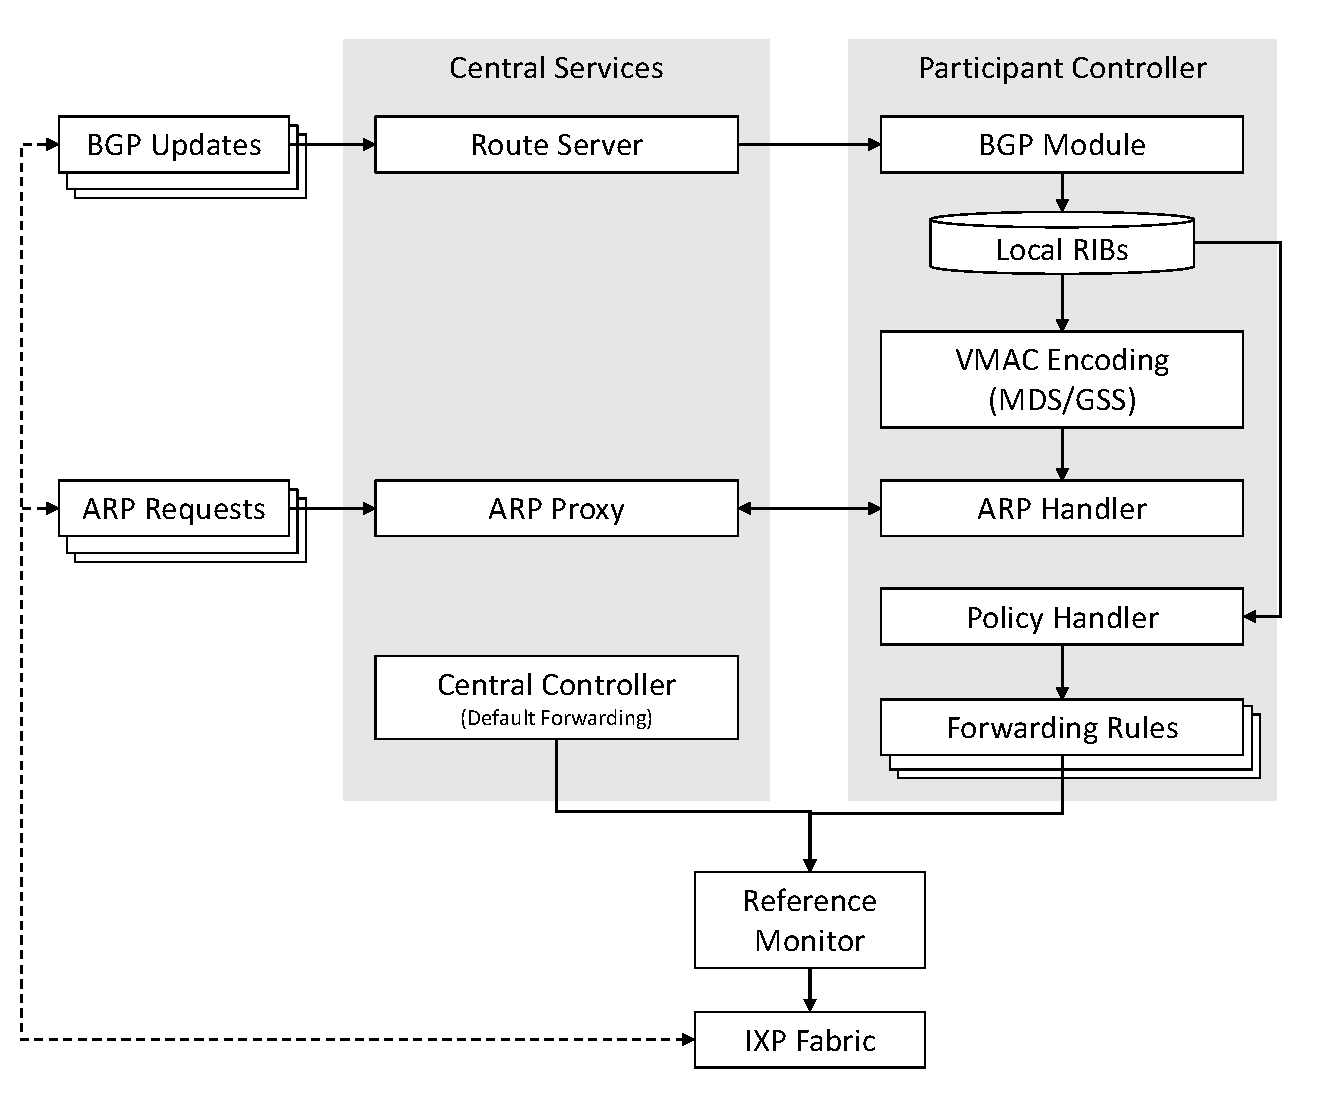
\includegraphics[scale = 0.4]{Figures/bckdgrnd_sdx_architecture_cropped.pdf}
\caption{iSDX architecture}
\end{figure}

The iSDX architecture has two main Parts. The Central Services and the Participant Controller. \\
Central Services forwards BGP updates and ARP queries to the corresponding participant controller. It also initializes all the static flow rules. \\
Every participant has its own participant controller. The participant controller receives and processes BGP updates from the Route Server. Every participant controller has a local routing information base keeping track of all the received routes, currently used routes and routes advertised to other participants.It takes care of the Virtual next-hop and VMAC assignment. It also updates policy flow rules and manages ARP requests and gratuitous ARP. Before BGP updates get sent to the participants border router they are processed by the participant controller.

\subsection{\label{chapter2:iSDX:policies}Policies}
Policies match on a field of the packet header and then forward the packet to a participant. Policies are implemented as flow rules that the participants controller programs into the SDN switch. 
\paragraph{\label{chapter2:iSDX:policies:outbound policies}Outbound Policies:}
Outbound policies let participants direct packets going from themselves to the iSDX. They allow the participants to choose the participant the packet gets sent to. An expamle of outbound policies is shown in Figure~\ref{fig:isdx_policies}, where participant A has defined two outbound policies directing traffic to either one of the other two participants.  

\paragraph{\label{chapter2:iSDX:policies:inbound policies}Inbound Policies:}
Inbound policies allow participants to direct packets coming from the iSDX. In effect they allow the participant to choose to which of his own routers packets from the iSDX get sent to. An example of inbound policies is shown in Figure~\ref{fig:isdx_policies}, where participant C has defined two inbound policies directing traffic to either one of it's routers. 

\begin{figure}[h]
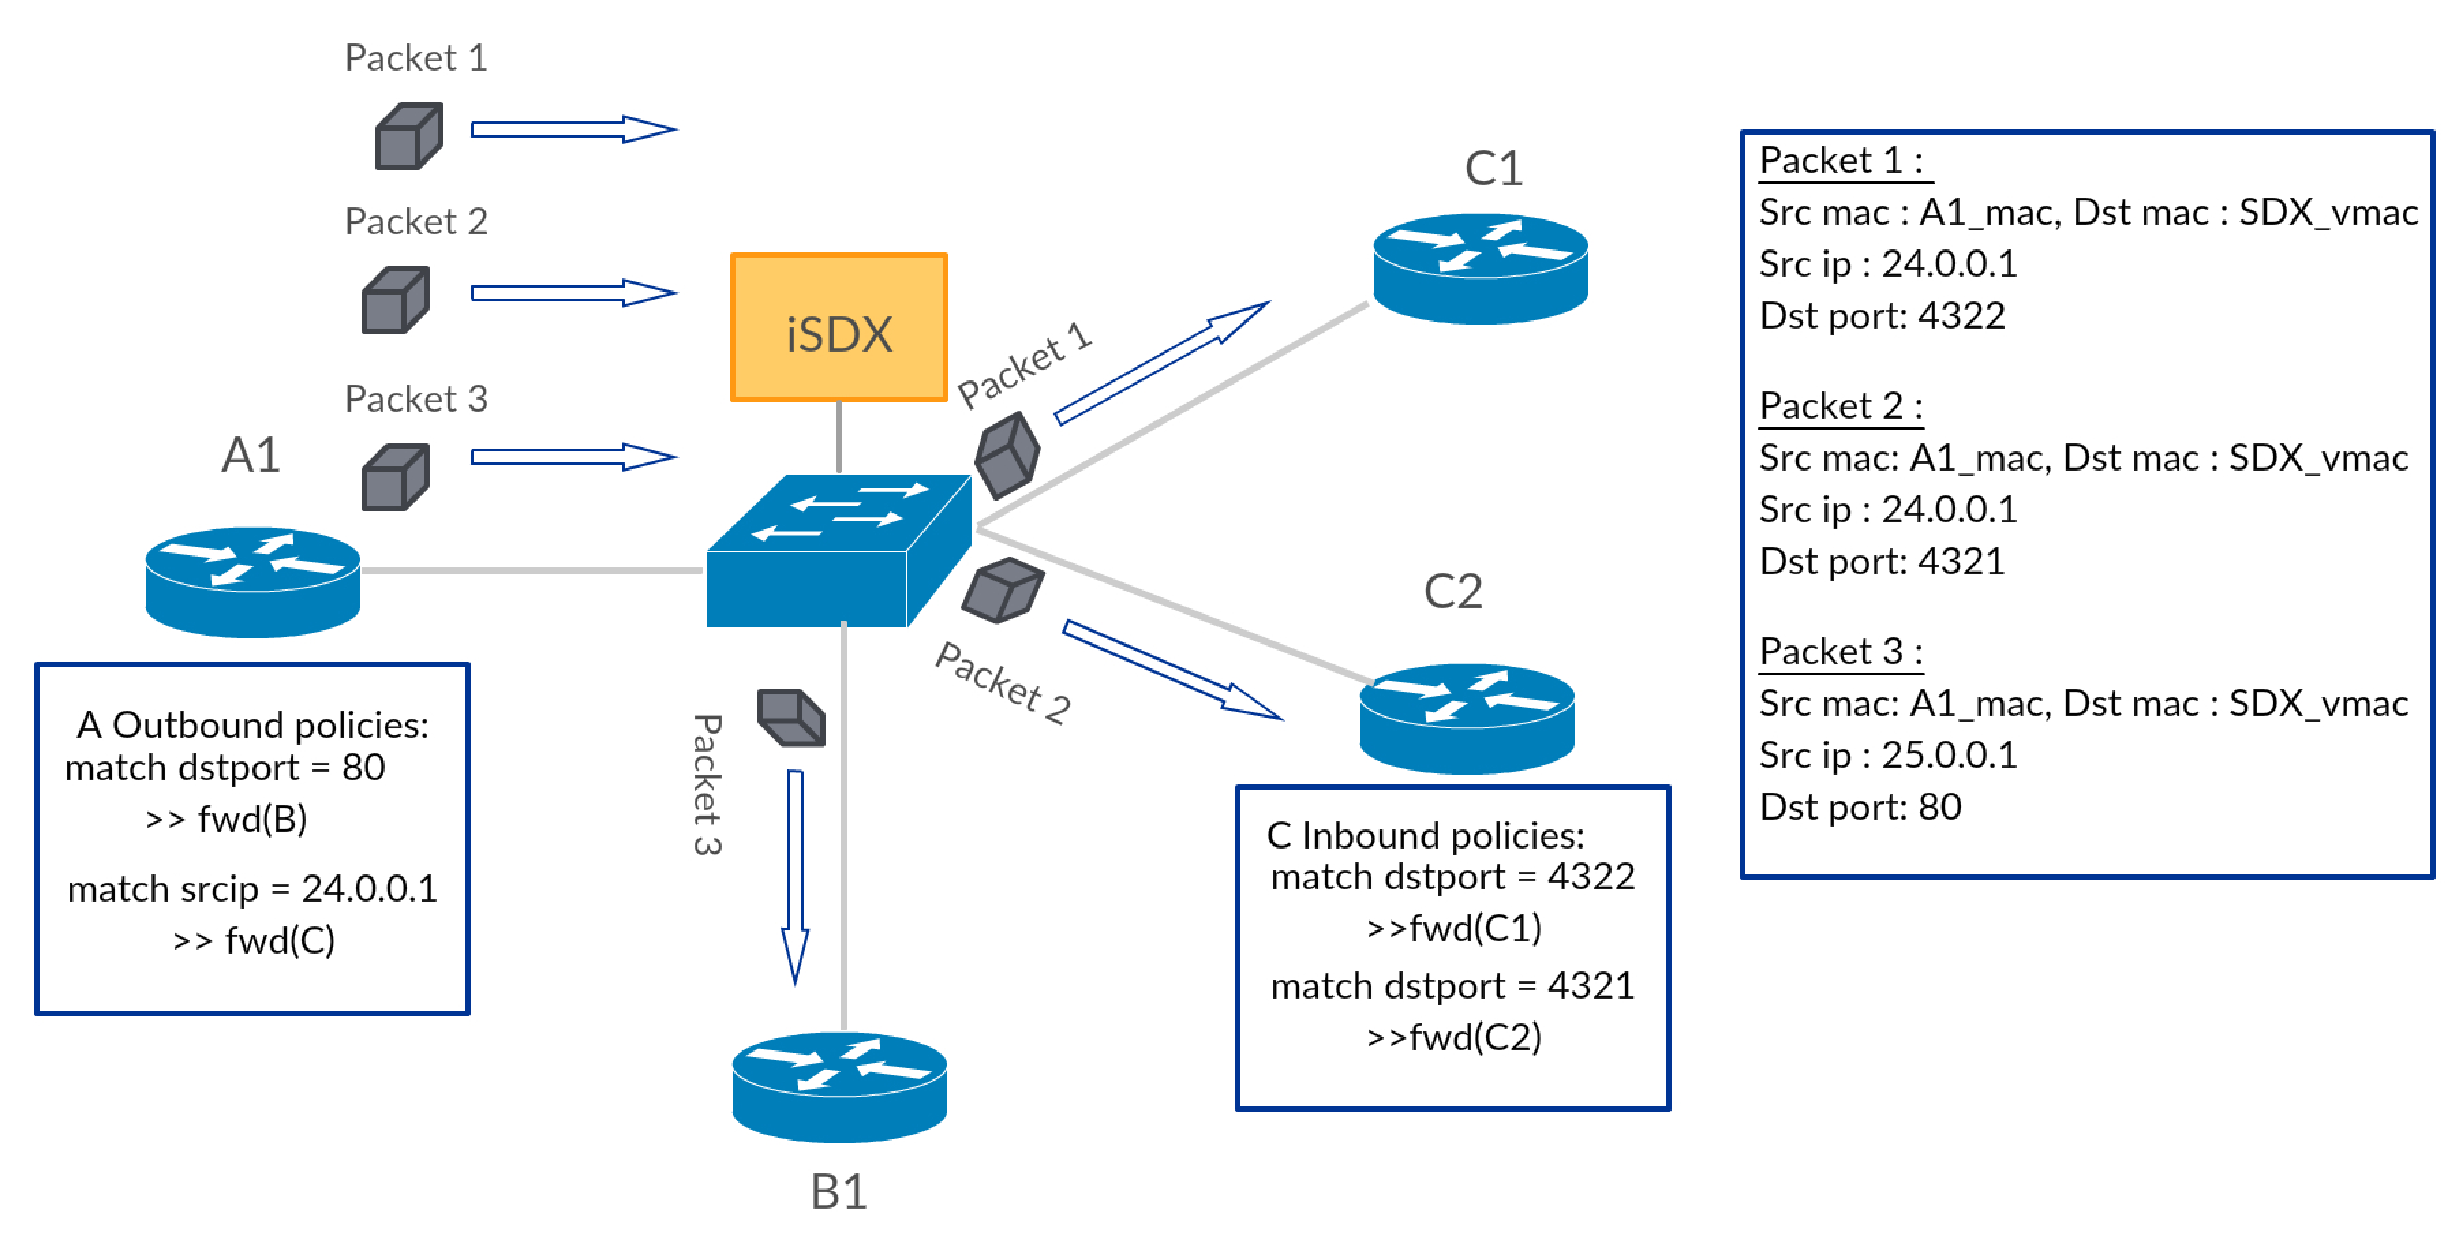
\includegraphics[scale = 0.32]{Figures/bckgrnd_sdx_policies.pdf}
\caption{Example of outbound and inbound policies with an iSDX connected to three \\ participants}
\label{fig:isdx_policies}
\end{figure}
  

\subsection{\label{chapter2:iSDX:VNH_VMAC}Virtual Next-Hop, Virtual MAC Address}


Participants are not restricted when defining outbound policies. Some policies might direct packets to participants that did not advertise the prefix or simply do not know a route to the prefix. This is a problem because outbound policies can end up violating BGP advertisements. The iSDX solves this problem by attaching additional information to each packet. This additional information is embedded into the destination mac address, transforming the destination mac addresses of packets traversing the SDN switch into a Virtual Mac Address. \\ 
In the Virtual Mac Address the participant controller encodes the participants advertising the prefix of the packet and the BGP best next hop participant for this prefix. The first part is used every time a outbound policy is applied. The outbound policy checks if the participant the outbound policy is sending packets to has advertised the prefix. The second part is used if the packet does not match any outbound policy. Default rules in the SDN switch match on the best next-hop participant and send the packet to this participant. \\
The Virtual Mac Address corresponds to a Virtual Next Hop, which is assigned to every prefix. \\ The participant controller sends BGP updates to it's border routers, with the next-hop of the update set to the Virtual Next-Hop of the prefix. The Virtual Mac Address is communicated to the participants via ARP. \\
Figure~\ref{fig:isdx_vmac} shows the Virtual Next-Hops and Virtual MAC Addresses used by participant A.

\paragraph{\label{chapter2:iSDX:virtual next-hop :inbound policies}iSDX VMAC:}

\rb{replace with a figure like the one later in the report}
\begin{tabular}{|r|l|}
  \hline 
  participants advertising the prefix & BGP best next-hop participant \\
  \hline
\end{tabular}

\begin{figure}[h]
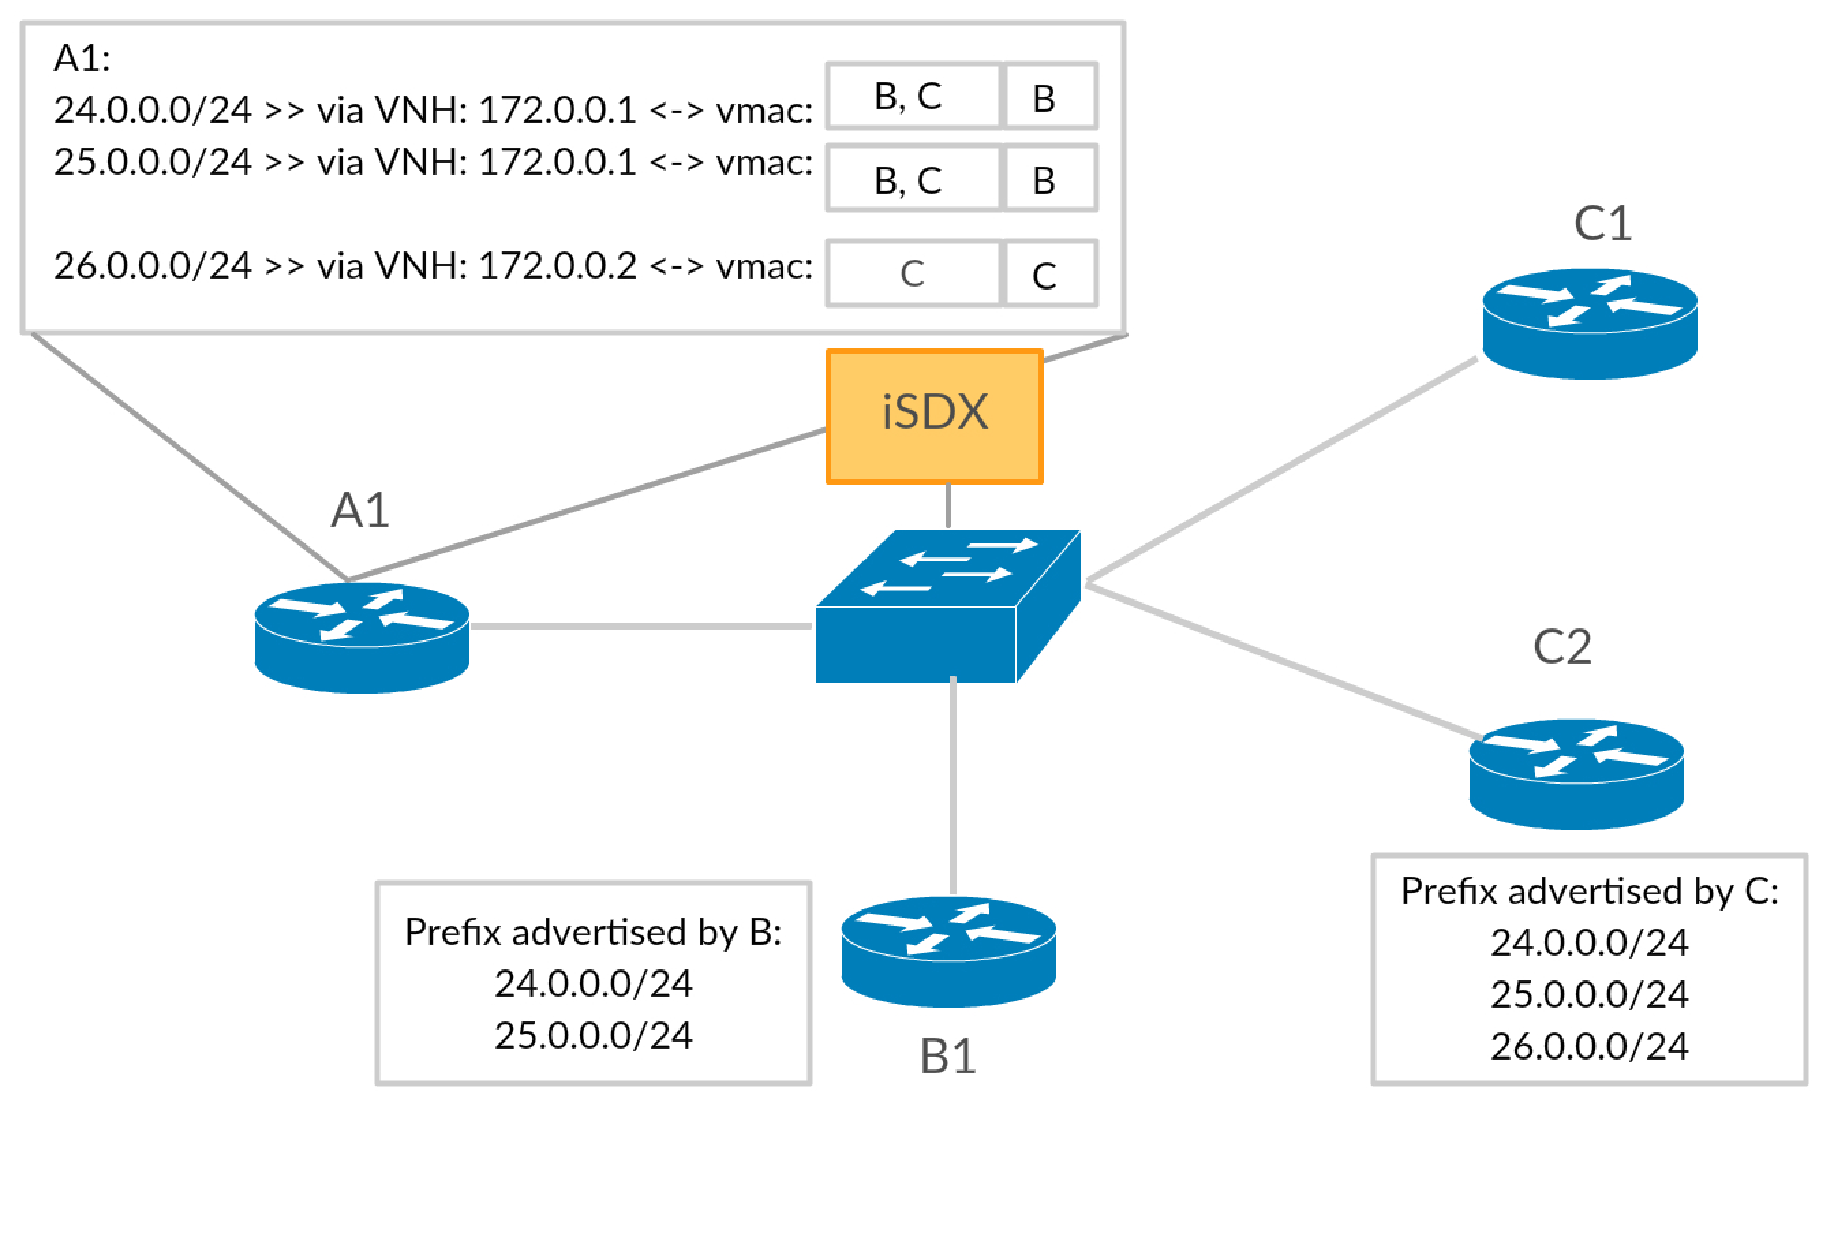
\includegraphics[scale = 0.36]{Figures/intro_sdx_vmac.pdf}
\caption{Example of the iSDX vmac with an iSDX connected to three participants}
\label{fig:isdx_vmac}
\end{figure}

\section{\label{chapter2:Swift}Swift}

\rb{make sure that the order of the iSDX and Swift text is aligned}

Swift is a prediction and fast-reroute framework to improve the convergence time of a BGP speaking router upon remote failure. Swifts prediction relies on the fact that the cause of a burst of withdrawals can be predicted before receiving all the withdrawals. \\
In this section we will show the Swift architecture in \ref{chapter2:Swift:Architecture_SWift}, explain the encoding in \ref{chapter2:Swift:encoding_of_routing_information} and how Swift reduces the convergence time of the swifted router in \ref{chapter2:Swift:BPA}.

\subsection{\label{chapter2:Swift:Architecture_SWift}Architecture}

\begin{figure}[h]
\center
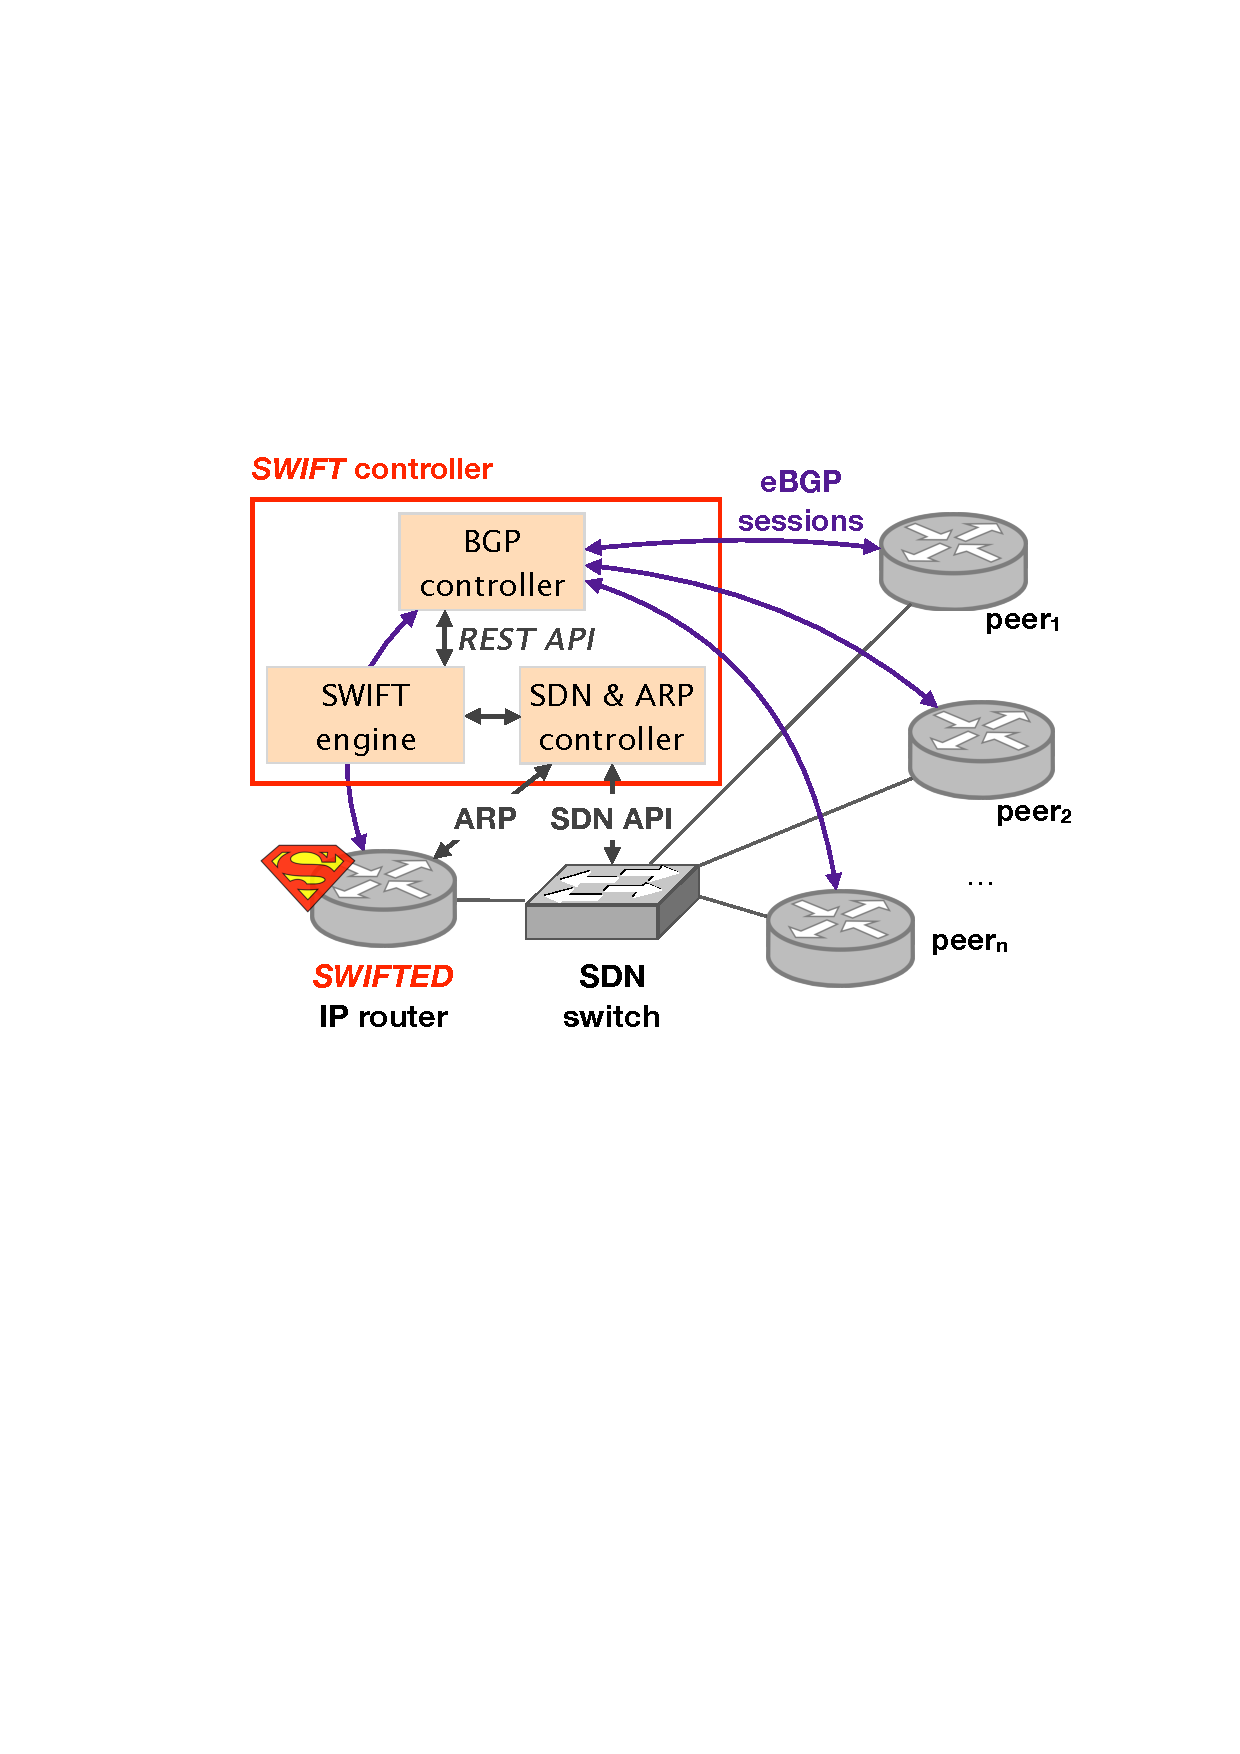
\includegraphics[scale = 0.5]{Figures/bckgrnd_swift_architecture.pdf}
\caption{Example topology of a swifted router}
\end{figure}

Swift uses a SDN switch connected to the swifted router, its neighbors and to the Swift controller. The Swift Controller has three main parts, the  BGP controller, Swift engine and the SDN \& ARP controller. The BGP controller receives BGP updates from the peers of the swifted router. The BGP controller forwards the updates to the Swift engine. The Swift engine has two main modules: the burst prediction algorithm and the encoding of routing information. These two modules are the two main features of Swift. The SDN \& ARP controller programs flow rules into the SDN switch and manages ARP requests. 


\subsection{\label{chapter2:Swift:encoding_of_routing_information}Encoding of Routing Information}
Swift similarly to the iSDX uses virtual next-hops and the destination mac address to encode information about the packet's prefix.\\
For every prefix Swift encodes the AS-path up to a certain depth and the backup next-hops for each AS-link on that AS-path. Backup next-hops are neigbhors of the swifted router which also advertise the prefix and their advertised route does not traverse the specific AS-link. This encoding is then mapped to a virtual next-hop. When the swifted router wants to send a packet to any prefix it will use the virtual next-hop assigned by Swift. The virtual next-hop directly maps to the destination mac address. \\
Figure~\ref{fig:isdx_vmac} shows the swifted router and the VMACs used for the prefixes advertised by the neigbhors.

\paragraph{\label{chapter2:Swift:Swift vmac}Swift VMAC:}

\begin{tabular}{|r|l|}
  \hline 
  backup next-hops for AS-links & AS-path \\
  \hline
\end{tabular}


\begin{figure}[h]
\center
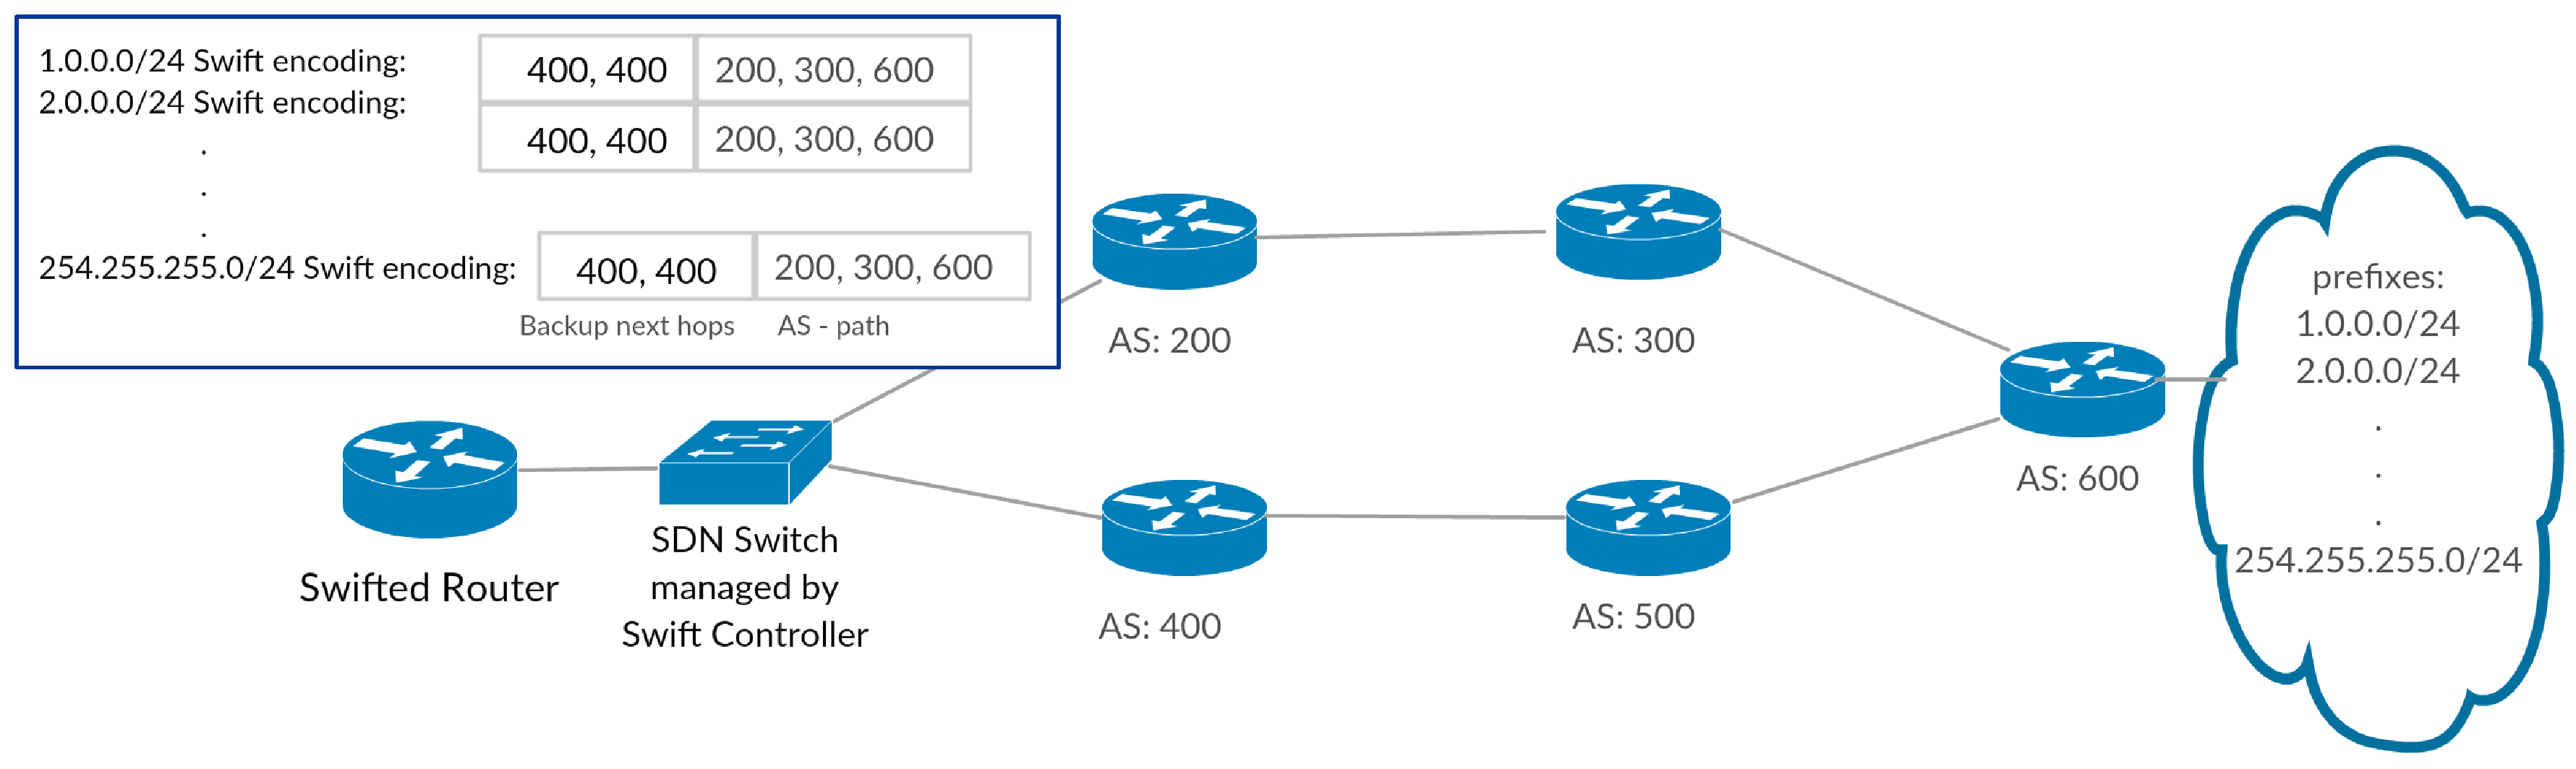
\includegraphics[scale = 0.24]{Figures/bckgrnd_swift_topology.pdf}
\caption{Example of the Swift vmac}
\label{fig:swift_vmac}
\end{figure}


\subsection{\label{chapter2:Swift:BPA}Burst Prediction Algorithm}
\rb{refer to the figure}
The burst prediction algorithm takes BGP updates. It uses the updates to build an AS-topology. Once enough withdrawals arrive in a time frame short enough to trigger a burst, the burst prediction algorithm uses the withdrawals and the AS-topology to predict the failed AS-link. \\
Upon predicting a failed link the Swift Controller pushes Fast Reroute flow rules into the SDN switch matching on the failed AS-link and on the corresponding backup next-hop. In Figure~\ref{fig:isdx_vmac} the burst prediciton module has predicted the AS-link 300 600 to be down. So it pushes rules matching on the AS-path 300 600 and the backup next-hop in this case 400.\\
Every packet that traverses the failed link (has the failed AS-link in it's AS-path encoding) will get rerouted to the backup neighbor.
\begin{figure}[h]
\center
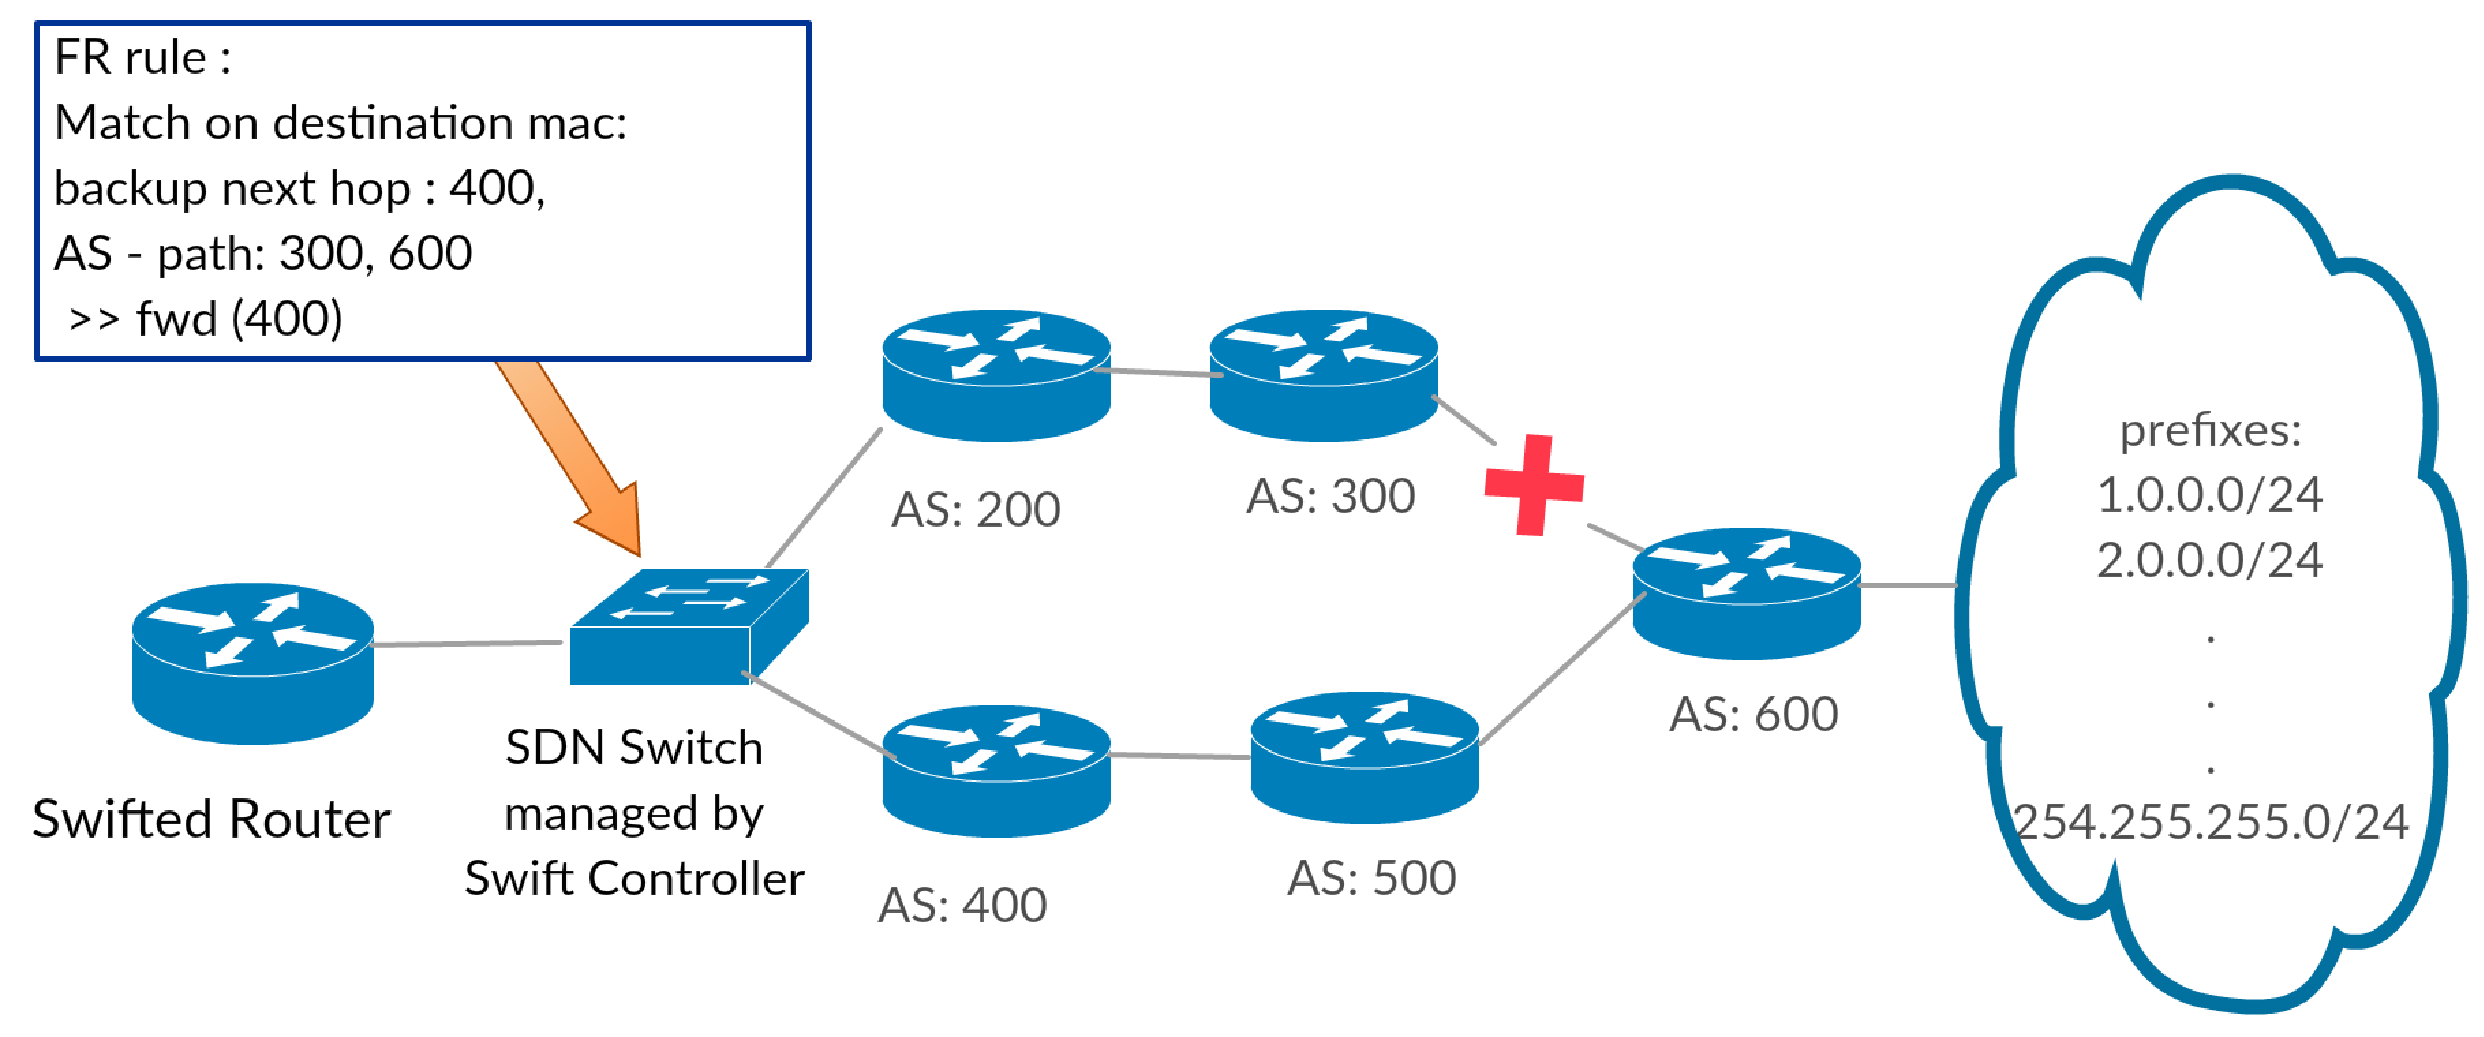
\includegraphics[scale = 0.36]{Figures/bckgrnd_swift_fr.pdf}
\caption{Example of a fast-reroute after BPA predicts the AS link 300 600 to be down}
\label{fig:swift_FR}
\end{figure}

By predicting the failed link and pushing Fast-Reroute rules instead of waiting for all withdrawals to arrive, Swift reduces the convergence time of the swifted router significantly.





